% ----------------------------------------------------------------------
% Provides ApplicationR for 'gems.tex' if R needed
% ----------------------------------------------------------------------
% Author: Thomas Gsponer, ISPM, Uni Bern
%         <tgsponer@ispm.unibe.ch>
% ----------------------------------------------------------------------
% Last modified: 14.01.2013
% ----------------------------------------------------------------------
% use: 
%%% setwd("C:/Users/nblaser/Documents/Cohort Model/JSS manuscript/sweave")
%%% Sweave("use.Rnw")
%
% Set global Sweave options:
% - use R engine;
% - do not create eps figures;
% - create pdf figures;


% Set further Sweave options:
% - use prefix.string as prefix for \includegraphics and include
%   the figure.


% This should handle the size of the figures.
% !!! NOT SURE EXACTLY HOW AND WHETHER IT WORKS !!!
\setkeys{Gin}{width=.9\textwidth}

% ----------------------------------------------------------------------
% Initialise R session for this section



%--------------------------------------------------------------------------------
% Using the package
%--------------------------------------------------------------------------------
\section[Using the package]{Using \pkg{gems}}\label{use}
In this section we illustrate how to use \pkg{gems} \citep{pkg:gems}. Figure~\ref{fig:flow} shows a flowchart of the steps to take to use \pkg{gems} and indicates where these steps are described in detail. First, Section~\ref{spec} shows how to specify all the necessary input (number of states, hazard functions and parameters) to run a simulation. Then Section~\ref{usesim} shows how to simulate from this input. Section~\ref{subsec:unc} describes how to include parameter covariances in the model and Section~\ref{subsec:bl} shows how to add baseline covariates. Finally Section~\ref{subsec:hist} describes how to include history dependence in the hazard functions and Section~\ref{subsec:ttt} describes an alternative to using hazard functions for specifying the transitions. 

% Define block styles
\tikzstyle{decision} = [diamond, draw, fill=blue!20, aspect=2.5, 
    text width=4.5em, text badly centered, inner sep=0pt]
    
\tikzstyle{stop} = [rectangle, draw, fill=blue!20, text width=5em, text centered, 
    rounded corners, minimum height=4em]
    
\tikzstyle{block} = [rectangle, draw, fill=blue!20, 
    text width=5em, text centered, minimum height=4em]
          
\tikzstyle{input} = [trapezium, trapezium left angle=70, trapezium right angle=-70, draw, fill=blue!20, 
    text width=5em, text centered, minimum height=4em]
    
\tikzstyle{line} = [draw, -latex']

\tikzstyle{start} = [draw, ellipse,fill=blue!20, node distance=3cm,
    minimum height=4em]
    
\tikzstyle{colcode} = [draw, circle, node distance=2cm, minimum height=4em]
    
\begin{figure}%
\begin{tikzpicture}[node distance = 2cm, auto]
    % Place nodes
    \node [start] (start) {Load gems};
    \node [input, below of=start, fill=green!20] (states) {Specify number of states};
    
    \node [block, below of=states, fill=green!20] (hazmat) {Generate hazard matrix};
    \node [input, below of=hazmat, fill=green!20] (haz) {Specify hazard functions};
    
    \node [block, below of=haz, fill=green!20] (parmat) {Generate parameter matrix};
    \node [input, below of=parmat, fill=green!20] (par) {Specify model parameters};
    
    \node [decision, below of=par, fill=yellow!20] (uncertain) {Model uncertainty?};
    \node [block, right of=uncertain, node distance=5cm, fill=yellow!20] (covmat) {Generate covariance matrix};
    \node [input, right of=covmat, node distance=5cm, fill=yellow!20] (cov) {Specify parameter covariances};
    
    \node [decision, below of=uncertain, , fill=orange!20] (baseline) {Include baseline?};
    \node [input, right of=baseline, node distance=5cm, fill=orange!20] (bl) {Specify characteristics};
    
    \node [block, below of=baseline, fill=red!20] (sim) {Simulate cohort};
    \node [stop, below of=sim] (end) {Analyse cohort};
%    % Draw edges
    \path [line] (start) -- (states);
    \path [line] (states) -- (hazmat);
    \path [line] (hazmat) -- (haz);
    \path [line] (haz) -- (parmat);
    \path [line] (parmat) -- (par);
    \path [line] (par) -- (uncertain);
    \path [line] (uncertain) -- node {yes} (covmat);
    \path [line] (covmat) -- (cov);
    \path [line] (uncertain) -- node {no}(baseline);
    \path [line] (baseline) -- node {yes} (bl);
    \path [line] (baseline) -- node {no}  (sim);
    \path [line] (sim) -- (end);
    % 
    \path [line] (bl) |- (sim);
    \path [line] (cov) |- ([yshift=1.72cm, xshift=0.9cm] baseline.south)
                       -- ([yshift=1.09cm, xshift=0.9cm] baseline.south);
                       
		% color code
		\node [colcode, below of=end, fill=blue!20, node distance=3cm] (blue) {\tiny Other};
		\node [colcode, right of=blue, fill=green!20] (green) {\tiny Section 3.1};
		\node [colcode, right of=green, fill=yellow!20] (yellow) {\tiny Section 3.3};
		\node [colcode, right of=yellow, fill=orange!20] (orange) {\tiny Section 3.4};
		\node [colcode, right of=orange, fill=red!20] (red) {\tiny Section 3.2};
		% shape code
%		 \node [start, below of=blue, fill=white] (start.shape) {\tiny Start};
%		 \node [block, right of=start.shape, fill=white] (block.shape) {\tiny Process};
%		 \node [input, right of=block.shape, fill=white, minimum height=1em] (input.shape) {\tiny Input};
%		 \node [decision, right of=input.shape, fill=white] (decision.shape) {\tiny Decision};
%		 \node [stop, right of=decision.shape, fill=white] (stop.shape) {\tiny Stop};
		 
		
\end{tikzpicture}
\caption{Flow chart indicating the steps users should take to simulate cohorts. The colors indicate where more detailed information is available. The parallelograms represent that user input is required, the rectangles represent that a process of \pkg{gems} performs this step and the diamonds represent user decisions.}%
\label{fig:flow}%
\end{figure}


The package is available at CRAN and can be loaded by

\begin{Schunk}
\begin{Sinput}
R> require("gems")
\end{Sinput}
\end{Schunk}

The package \pkg{gems} uses three classes to encode all model inputs and outputs.
\begin{enumerate}
  \item A \code{transition.structure} contains the number of model states and a \code{matrix} with elements that are used to specify transition-specific hazard functions, their parameters and covariances. 
  \item An \code{ArtCohort} contains all aspects of the simulated cohort, including the model input and a \code{data.frame} with the entry times for each patient into each of the states. 
  \item The \code{PosteriorProbabilities} contain the transition probabilities or cumulative incidence that can be calculated from the \code{ArtCohort}.
\end{enumerate}

The model has six main functions. The first three are used to specify the model, the fourth is used for simulation and the last two are used to summarize the results. 
\begin{enumerate}
  \item \code{generateHazardMatrix} creates a template of class
    \code{transition.structure} that can be used to specify the transition-specific hazard functions. 
  \item \code{generateParameterMatrix} creates a template of class \code{transition.structure} that can be used to specify the parameters.
  \item \code{generateParameterCovarianceMatrix} creates a \code{transition.structure} that can be used to specify the parameter covariance. 
  \item \code{simulateCohort} simulates the specified artificial cohort and returns an object of class \code{ArtCohort}.
  \item \code{transitionProbabilities} returns an object of class
    \code{posteriorProbabilities} that contains the transition probabilities from the initial state over time.
  \item \code{cumulativeIncidence} returns an object of class
    \code{posteriorProbabilities} that contains the cumulative incidence over time.
\end{enumerate}

\subsection[Model specification]{Specifying the model}\label{spec}

Suppose we want to simulate a disease with initial state $E_1$, intermediate state $E_2$ and absorbing state $E_3$ as depicted in the DAG in Figure~\ref{fig:specDAG}.
\begin{figure}[htb!] 
		\centering
		\setlength{\unitlength}{2mm}
		\begin{picture}(50,20)(5,10)
		
		% Stages before Switch
		\put(10, 15){\circle{7.5}}
		\put(8.8,14){$E_1$}
		
		\put(30, 25){\circle{7.5}}
		\put(28.8,24){$E_2$}
%		\put(30, 5){\circle{7.5}}
%		\put(27.8,3.8){$E_3$}
	
		\put(50, 15){\circle{7.5}}
		\put(48.8,14){$E_3$}
	
		% Transitions
		\put(13.35, 16.68){\vector(2,1){13.29}}
%		\put(13.35, 13.32){\vector(2,-1){13.29}}
		
		\put(13.75, 15){\vector(1,0){32.5}}
	
%		\put(33.35, 6.68){\vector(2,1){13.29}}
		\put(33.35, 23.32){\vector(2,-1){13.29}}
		
		% Hazards
		\put(18, 23){\text{$h_{12}(t)$}}
		\put(38, 23){\text{$h_{23}(t)$}}
		
		\put(27.8, 16){\text{$h_{13}(t)$}}

%		\put(18, 5.5){\text{$h_{13}$}}
%		\put(38, 5.5){\text{$h_{34}$}}
	
		\end{picture}
		\caption[Model specification DAG]{\label{fig:specDAG} Model specification DAG.}
\end{figure}
In order to fully specify the model, the hazard functions, their parameters and the covariance structure of these parameters must be specified. The hazard functions are specified in a \code{transition.structure} of dimension $states \times states$. 

The function \code{generateHazardMatrix} can be used to specify such a \code{transition.structure} that contains only the model structure. 
\begin{Schunk}
\begin{Sinput}
R>   hf <- generateHazardMatrix(3)
R>   print(hf)
\end{Sinput}
\begin{Soutput}
         to
from      State 1 State 2      State 3     
  State 1 NULL    "impossible" "impossible"
  State 2 NULL    NULL         "impossible"
  State 3 NULL    NULL         NULL        
\end{Soutput}
\end{Schunk}
% str(hf)
The argument \code{statesNumber} specifies the number of states in the multistate model. The resulting \code{transition.structure} only provides the basic structure for how hazard functions are specified and the desired hazard functions must be entered. 

For exponential, Weibull and Weibull mixture distributions, the built-in functions can be specified as \code{"Exponential"}, \code{"Weibull"}, and \code{"multWeibull"} respectively. Arbitrary continuous hazards can also be specified as functions. 

For instance, assume that the transition times $T_{12}$ and $T_{13}$ are exponentially distributed and the transition time $T_{23}$ is Weibull distributed. Then the \code{transition.structure} can be set up using double square brackets as follows. 
To show different ways of specifying time-to-event distributions, we used a user-supplied function for $T_{12}$ and a built-in function for $T_{13}$, even though they are both exponentially distributed. 
For the first transition, the hazard function of an exponential is specified as a hazard function with its own parameterization. The parameterization of the built-in functions is explained below. Note that user-supplied functions need to return a result of the same length as the time argument $t$. The required code to specify the hazard functions described above is
\begin{Schunk}
\begin{Sinput}
R>   hf[[1, 2]] <- function(t, mu) rep(1 / mu, length(t))
R>   hf[[1, 3]] <- "Exponential"
R>   hf[[2, 3]] <- "Weibull"
R>   print(hf)
\end{Sinput}
\begin{Soutput}
         to
from      State 1 State 2           State 3      
  State 1 NULL    "function(t, mu)" "Exponential"
  State 2 NULL    NULL              "Weibull"    
  State 3 NULL    NULL              NULL         
\end{Soutput}
\end{Schunk}
When specifying a function as \code{"Exponential"} or \code{"Weibull"}, the parameterization is the same as in the \code{rexp} or \code{rweibull} function; that is,
\begin{align} \label{eqn:ExpWeib_param}
  h_{exp}(t, rate) &= rate, \\
  h_{Weibull}(t, shape, scale) &= \frac{shape}{scale} \left( \frac{t}{scale} \right)^{shape-1}. 
\end{align}
For the Weibull mixture model, the parameterization is
\begin{align} \label{eqn:MultWeib_param}
  h_{multWeibull}(t, \bm\omega, \mathbf{k}, \bm\lambda) = 
    \frac{\omega_1 f_W(t, k_1,  \lambda_1) + \dots + \omega_n f_W(t, k_n, \lambda_n)}
    {\omega_1 (1-F_W(t, k_1, \lambda_1)) + \dots + \omega_n (1-F_W(t, k_n, \lambda_n))}, 
\end{align}
where $f_W$ and $F_W$ are the Weibull density and distribution functions in the same parameterization as before, where $k_i$ is the shape and $\lambda_i$ the scale of the $i$-th Weibull distribution. Here $\mathbf{k}$ and $\bm\lambda$ are $n$-dimensional vectors and $\bm\omega$ is an $(n-1)$ dimensional vector with $\omega_n = 1-\sum_{i=1}^{n-1} \omega_i$ being defined automatically. Mixed Weibull distributions can be used when there are multiple modes of failure that result in the same state and can be estimated using maximum likelihood or non-linear least squares methods \citep{Ling2009}.

Specifying built-in functions is more efficient than specifying the hazard function of a Weibull distribution, because the simulation internally uses \code{rweibull} instead of using piecewise approximation of the Weibull hazard function and \code{rpexp} to generate Weibull distributed random numbers. 

Once all hazard functions are suitably specified, the parameter values must be determined. The easiest way to do this is by using the function \code{generateParameterMatrix}, with the hazard structure \code{hf} as an argument,
\begin{Schunk}
\begin{Sinput}
R>   par <- generateParameterMatrix(hf)
R>   par[[1, 2]] <- list(mu = 3.1)
R>   par[[1, 3]] <- list(rate = 0.3)
R>   par[[2, 3]] <- list(shape = 3, scale = 3)
\end{Sinput}
\end{Schunk}
The \code{transition.structure} generated by \code{generateParameterMatrix} is again only a framework; the specific parameter values need to be assigned afterwards. Note that the parameters need to be specified in the order in which they appear in the function. 
%Names like shape and scale in the list are not meant to match with the internal definitions for Weibull associated functions, but we recommend its use for more convenience. 

\subsection[Simulation]{Simulation and post-processing}\label{usesim}

Once the model is specified, the simulation can be invoked with the \code{simulateCohort} function. The arguments for \code{simulateCohort} are the previously specified \code{transitionFunction}, \code{parameters}, as well as the number of patients \code{cohortSize} to be simulated and the final time \code{to} of the simulation.
\begin{Schunk}
\begin{Sinput}
R>   cohortSize <- 10000
R>   cohort <- simulateCohort(transitionFunctions = hf, 
+                            parameters = par, 
+                            cohortSize = cohortSize, 
+                            to = 10)
R>   head(cohort)
\end{Sinput}
\begin{Soutput}
          State 1   State 2   State 3
Patient 1       0        NA 2.8115242
Patient 2       0 4.3985589 8.7294035
Patient 3       0        NA 2.5803986
Patient 4       0        NA 0.2123987
Patient 5       0 0.5824707 4.5493082
Patient 6       0        NA 2.6388907
\end{Soutput}
\end{Schunk}
The output \code{ArtCohort} contains the entry time into the different states for each patient. 

Next, we can calculate and plot the transition probabilities and cumulative incidence including $95\%$ confidence intervals from the initial state using the functions \code{transitionProbabilities} and \code{cumulativeIncidence} respectively.
\begin{Schunk}
\begin{Sinput}
R>   post <- transitionProbabilities(cohort, times = seq(0,5, .1))
R>   cinc <- cumulativeIncidence(cohort, times = seq(0,5, .1))
R>   head(post)
\end{Sinput}
\begin{Soutput}
         State 1 State 2 State 3
Time 0    1.0000  0.0000  0.0000
Time 0.1  0.9384  0.0344  0.0272
Time 0.2  0.8808  0.0658  0.0534
Time 0.3  0.8272  0.0933  0.0795
Time 0.4  0.7775  0.1187  0.1038
Time 0.5  0.7272  0.1464  0.1264
\end{Soutput}
\begin{Sinput}
R>   head(cinc)
\end{Sinput}
\begin{Soutput}
         State 1 State 2 State 3
Time 0         1  0.0000  0.0000
Time 0.1       1  0.0344  0.0272
Time 0.2       1  0.0658  0.0534
Time 0.3       1  0.0933  0.0795
Time 0.4       1  0.1188  0.1038
Time 0.5       1  0.1465  0.1264
\end{Soutput}
\end{Schunk}
\begin{Schunk}
\begin{Sinput}
R>   plot(post, main = "Transition probabilities", ci = TRUE)
\end{Sinput}
\end{Schunk}
\begin{Schunk}
\begin{Sinput}
R>   plot(cinc, main = "Cumulative incidence", ci = TRUE)
\end{Sinput}
\end{Schunk}

For the \code{transitionProbabilities} function, the argument \code{times} specifies the timepoints at which the transition probabilities should be returned. The \code{plot} function admits the argument \code{ci} in order to add confidence intervals to the figure. Figure~\ref{fig:postProb} shows the transition probabilities and Figure~\ref{fig:cincProb} shows the cumulative incidence in the above example. 

\begin{figure} 
\begin{center}
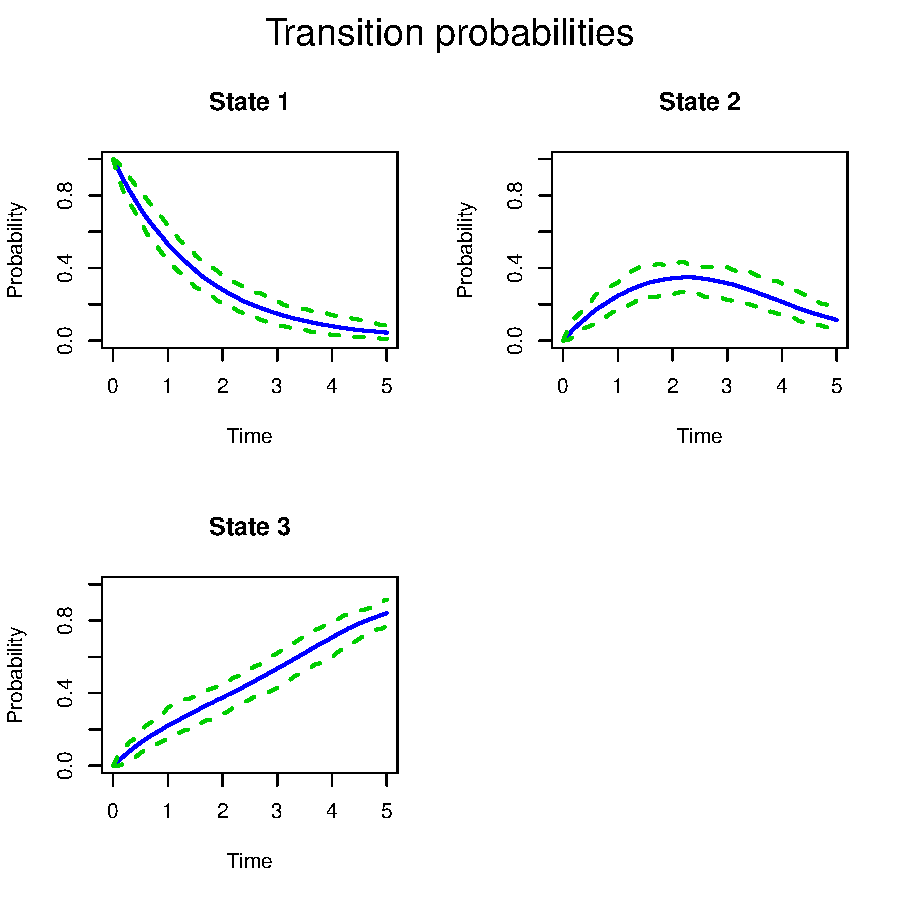
\includegraphics{PDF/Application-postPlot}
\end{center}
\caption{Transition probabilities.}
\label{fig:postProb}
\end{figure}

\begin{figure} 
\begin{center}
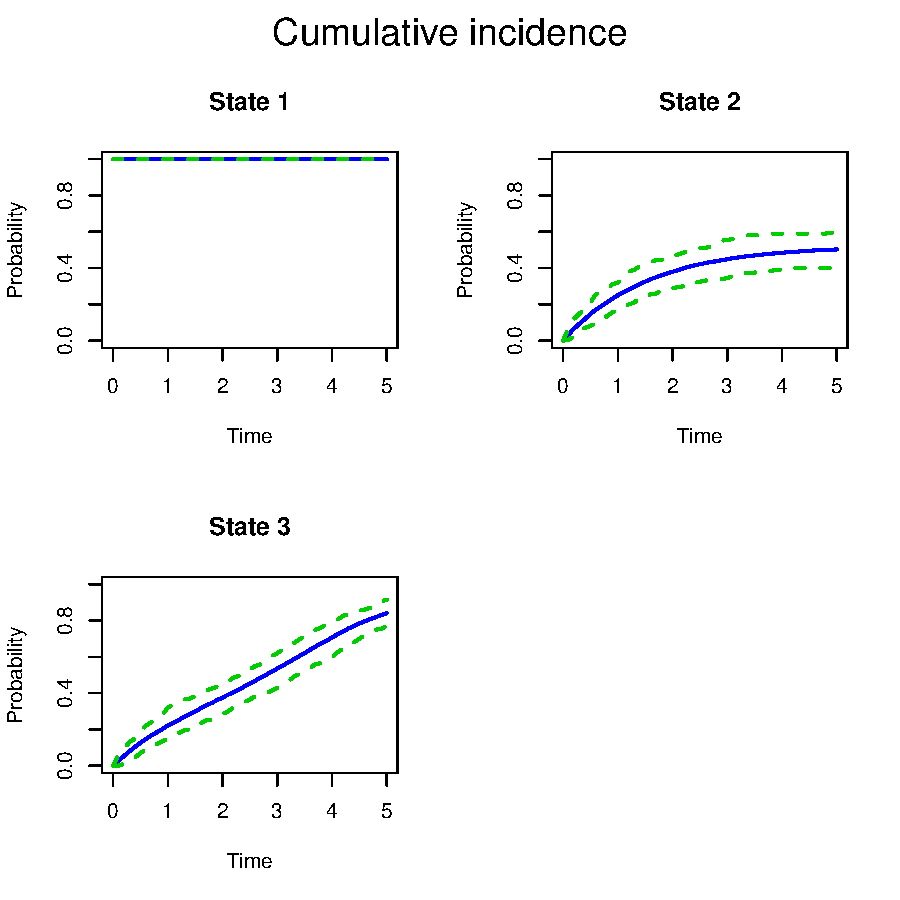
\includegraphics{PDF/Application-cincPlot}
\end{center}
\caption{Cumulative incidence.}
\label{fig:cincProb}
\end{figure}

\subsection{Parameter uncertainty}\label{subsec:unc}
Suppose that we want to include parameter uncertainty in the above example. For instance, we estimate the shape and scale parameters for the transition from $E_2$ to $E_3$ be distributed as follows:
\begin{align} \label{eqn:unc}
  \begin{pmatrix}
    shape \\ scale 
  \end{pmatrix}
  \sim
  \mathcal{MN}\left( 
    \begin{pmatrix}
      3 \\ 3 
    \end{pmatrix}
    ,
    \begin{pmatrix}
      0.5 & 0 \\ 0 & 0.5
    \end{pmatrix}
  \right) .
\end{align}

Then the covariance matrix can be specified using the \code{generateParameterCovarianceMatrix} function with the previously generated parameter \code{transition.structure} as an argument.
\begin{Schunk}
\begin{Sinput}
R>   cov <- generateParameterCovarianceMatrix(par)
R>   cov[[2, 3]] <- diag(.5, 2)
\end{Sinput}
\end{Schunk}
As with the parameter \code{transition.structure}, also the values of the parameter covariance \code{transition.structure} need to be specified after generating the \code{transition.structure}. 

For the simulation, the uncertainty is included in the \code{parameterCovariance} argument for \code{simulateCohort} as follow:
\begin{Schunk}
\begin{Sinput}
R>   cohort <- simulateCohort(transitionFunctions = hf, 
+                            parameters = par, 
+                            parameterCovariances = cov,
+                            cohortSize = cohortSize, 
+                            to = 10)
\end{Sinput}
\end{Schunk}


\subsection{Baseline characteristics}\label{subsec:bl}
Baseline characteristics can be included in the model by letting the hazard depend on the argument \code{baseline}; for example, if age and sex are important characteristics. 
Consider sex  to be encoded as $0$ for males and as $1$ for females, and let the baseline age be the age in years. Suppose we want to simulate a cohort of $50\%$ men and $50\%$ women with ages distributed uniformly between 20 and 50. Baseline characteristics should be specified in a \code{matrix} or \code{data.frame} as follows.
\begin{Schunk}
\begin{Sinput}
R>   bl <- data.frame(sex = rbinom(cohortSize, 1, .5), 
+                    age = runif(cohortSize, 20, 50))
R>   head(bl)
\end{Sinput}
\begin{Soutput}
  sex      age
1   0 21.02408
2   1 44.70358
3   0 20.70234
4   1 36.94189
5   0 48.42227
6   1 29.78793
\end{Soutput}
\end{Schunk}

If there is a sex-specific rate, one option would be to record it as a \code{numeric} of \code{length} $2$, with the first position describing the rate for male and the second position the rate for women. Suppose age is another risk factor, specified as a rate ratio per year. In this case the function would depend on the sex-specific rate \code{rate}, the rate ratio  \code{rr} per year of age and the baseline characteristics \code{bl}. The model could then be specified as follows. 
\begin{Schunk}
\begin{Sinput}
R>   hf[[1, 2]] <- function(t, bl, rate, rr) {
+     rep(rate[bl["sex"] + 1], length(t)) * rr ^ (bl["age"] - 20)
+   }
R>   par[[1, 2]] <- list(rate = c(0.2,0.3), rr = 1.02)
R>   cov[[1, 2]] <- diag(0, 3)
\end{Sinput}
\end{Schunk}

In order to simulate from this model that includes baseline characteristics, an additional argument \code{baseline} is added to the \code{simulateCohort} function as follows. 
\begin{Schunk}
\begin{Sinput}
R>   cohort <- simulateCohort(transitionFunctions = hf, 
+                            parameters = par, 
+                            cohortSize = cohortSize, 
+                            parameterCovariances = cov, 
+                            baseline = bl,
+                            to = 5)
\end{Sinput}
\end{Schunk}


\subsection{History dependence}\label{subsec:hist}
In many real-world applications, transitions between states may depend both on the current state, and on the history of previous events in the patient history. For instance, in an HIV treatment model, the immune system worsens between failure of first-line therapy and start of second-line treatment and the mortality hazard after starting a second-line therapy depends on how long a person spent on failing first-line treatment \citep{Gazzola2009}.

History-dependence of the model can be specified by letting the hazard function depend on the argument \code{history}. 
This \code{history}-argument is a vector indexed by the transition-number
\begin{Schunk}
\begin{Sinput}
R>   gems:::auxcounter(3)
\end{Sinput}
\begin{Soutput}
         to
from      State 1 State 2 State 3
  State 1       0       1       2
  State 2       0       0       3
  State 3       0       0       0
\end{Soutput}
\end{Schunk}
and is the transition time $T_i$ for the transitions that have occurred. For transitions that have not yet occurred, the \code{history} argument is $0$. 

The \code{history} argument allows to use the clock-forward approach (time refers to the time since the patient entered the initial state)  instead of the clock-reset approach (time refers to time since entry into current state) to multistate modeling \citep{Putter2007}. To use the clock-forward approach, \code{t} can be replaced by \code{t + sum(history)}. 
Note that the clock-forward approach does not support built-in function (\code{"Exponential"}, \code{"Weibull"} and \code{"multWeibull"}) and users have to supply their own functions. 
If the transition-specific hazard for transition $3$ was estimated using the clock-forward approach instead of the clock-reset approach, the Weibull function could be specified as follows.
\begin{Schunk}
\begin{Sinput}
R>   hf[[2, 3]] <- function(t, shape, scale, history) {
+     shape/scale * ((t + sum(history)) / scale) ^ (shape - 1)  
+   }
\end{Sinput}
\end{Schunk}
The \code{simulateCohort} function can be used with this new function just as it was before. 


\subsection{Time to transition functions}\label{subsec:ttt}
Sometimes it is easier not to specify transitions via their hazards, but to directly specify the time it takes until the transition occurs. For instance, in some cases test results need to be confirmed by a second test three months later (e.g., HIV treatment failure tests \citep{Estill2012}). Then the time would be three months and the hazard function would be a function with infinite point mass in 3. An additional argument \code{timeToTransition} to the \code{simulateCohort} function would have to be given by a \code{matrix}; the position of this kind of transition would be \code{TRUE} and the rest (usual hazard functions) would be \code{FALSE}. This procedure and the specification of the \code{transitionFunction} is as follows:
\begin{Schunk}
\begin{Sinput}
R>   hf[[1, 3]] <- function() 3
R>   par[[1, 3]] <- list()
R>   ttt <- matrix(FALSE, nrow = 3, ncol = 3)
R>   ttt[1, 3] <- TRUE
R>   cohort <- simulateCohort(transitionFunctions = hf, 
+                            parameters = par, 
+                            cohortSize = cohortSize, 
+                            parameterCovariances = cov, 
+                            timeToTransition = ttt,
+                            baseline = bl,
+                            to = 5)
\end{Sinput}
\end{Schunk}


